\documentclass[12pt,a4paper]{article}
\usepackage[margin=1in]{geometry}
\usepackage{parskip}
\usepackage{microtype}
\usepackage{booktabs}
\usepackage{graphicx}
\usepackage{amsmath,amssymb}
\usepackage[most]{tcolorbox}

\title{Fitting a Weibull to the period of $\sqrt{n}$}
\author{Robin Langer}
\date{}

\begin{document}
\maketitle
\vspace{-1.5em}

\section{The problem}

Every square root of a non square whole number repeats forever.

\begin{center}
\begin{tabular}{ll}
\toprule
$\sqrt{2}$  & $[\,1;\ \overline{2}\,]$ \\
$\sqrt{3}$  & $[\,1;\ \overline{1,2}\,]$ \\
$\sqrt{5}$  & $[\,2;\ \overline{4}\,]$ \\
$\sqrt{6}$  & $[\,2;\ \overline{2,4}\,]$ \\
$\sqrt{7}$  & $[\,2;\ \overline{1,1,1,4}\,]$ \\
$\sqrt{13}$ & $[\,3;\ \overline{1,1,1,1,6}\,]$ \\
$\sqrt{19}$ & $[\,4;\ \overline{2,1,3,1,2,8}\,]$ \\
$\sqrt{31}$ & $[\,5;\ \overline{1,1,3,5,3,1,1,10}\,]$ \\
$\sqrt{94}$ & $[\,9;\ \overline{1,2,3,1,1,5,1,8,1,5,1,1,3,2,1,18}\,]$ \\
\bottomrule
\end{tabular}
\end{center}

The notation $[a; b, c, d, \ldots]$ means the tower
\[
  a + \cfrac{1}{b + \cfrac{1}{c + \cfrac{1}{d + \cdots}}}
\]
and the bar marks the part that repeats. Write $L(n)$ for the length of that repeating block.

The length is not predictable from $n$. $\sqrt{61}$ needs eleven terms and $\sqrt{65}$ needs one. No formula gives it. So the question is statistical rather than exact: taken over many $n$, what distribution does the period follow?

$L(n)$ itself grows, roughly like $\sqrt{n}$, so the variable to study is the normalised one
\[
  t \;=\; \frac{L(n)}{\sqrt{n}} .
\]
Its density is a decaying curve with a soft right hand edge near $2.5$. It looks exponential. This document asks whether it is, and fits the natural one-parameter generalisation.

\section{The Weibull distribution}

Write $S(t) = P(X>t)$ for the survival function. The exponential and the Weibull sit side by side:
\[
  \text{exponential}\quad S(t) = e^{-t/\lambda},
  \qquad\qquad
  \text{Weibull}\quad S(t) = e^{-(t/\lambda)^k}.
\]
One extra exponent. Its meaning appears in the hazard rate $h(t)=f(t)/S(t)$, the instantaneous rate of stopping given that you have got this far:
\[
  \text{exponential}\quad h(t) = \frac{1}{\lambda},
  \qquad\qquad
  \text{Weibull}\quad h(t) = \frac{k}{\lambda}\Bigl(\frac{t}{\lambda}\Bigr)^{k-1}.
\]

So the Weibull is the distribution whose hazard is a power of $t$, and $k$ is that power.

\begin{center}
\begin{tabular}{ll}
\toprule
$k=1$ & constant hazard. The Weibull \emph{is} the exponential. Memoryless. \\
$k<1$ & falling hazard. Survive a while and you are more likely to continue. \\
$k>1$ & rising hazard. Wear-out; a soft edge ahead. \\
\bottomrule
\end{tabular}
\end{center}

It is the right second thing to try after an exponential because it adds exactly one parameter, and that parameter indexes the only feature the exponential refuses to have.

Note for later that $h$ is a power of $t$, hence \emph{monotone for every $k$}. A Weibull hazard can fall or rise. It cannot do one and then the other.

\section{Method}

\textbf{The period.} Generated by the PQa recurrence, which holds the surd in exact integers and never touches a float. With $a_0=\lfloor\sqrt n\rfloor$, $P_0=0$, $Q_0=1$,
\[
  a_i = \left\lfloor \frac{a_0+P_i}{Q_i} \right\rfloor,
  \qquad
  P_{i+1} = a_iQ_i - P_i,
  \qquad
  Q_{i+1} = \frac{n-P_{i+1}^2}{Q_i},
\]
and the block closes at the first $i\ge 1$ with $Q_i=1$. Every quantity is an integer, so there is no tolerance to choose and no accumulated error.

\textbf{The fits.} Maximum likelihood, with the location parameter fixed at $0$ since $t>0$ by construction. The exponential fit is then just the sample mean.

\textbf{The test.} Kolmogorov--Smirnov distance between the empirical and fitted distribution functions, compared against the $5\%$ critical value $1.358/\sqrt{N}$.

\textbf{The bands.} Seven disjoint ranges of $n$ from $10^4$ to $9\times 10^5$, each fitted separately, so that any drift in the fitted parameters is visible rather than averaged away.

\section{Results}

\begin{center}
\begin{tabular}{lrrrrrr}
\toprule
band & $N$ & mean $t$ & $k$ & KS exp & KS Weib & $5\%$ cut \\
\midrule
$[10^4,\,4\!\cdot\!10^4)$      & $29{,}900$ & $0.3872$ & $1.0369$ & $0.0222$ & $0.0214$ & $0.0079$ \\
$[5\!\cdot\!10^4,\,8\!\cdot\!10^4)$ & $29{,}941$ & $0.3632$ & $0.9961$ & $0.0248$ & $0.0239$ & $0.0078$ \\
$[10^5,\,1.3\!\cdot\!10^5)$    & $29{,}956$ & $0.3526$ & $0.9826$ & $0.0232$ & $0.0191$ & $0.0078$ \\
$[2\!\cdot\!10^5,\,2.3\!\cdot\!10^5)$ & $29{,}968$ & $0.3420$ & $0.9596$ & $0.0338$ & $0.0216$ & $0.0078$ \\
$[3\!\cdot\!10^5,\,4\!\cdot\!10^5)$   & $99{,}915$ & $0.3343$ & $0.9480$ & $0.0346$ & $0.0210$ & $0.0043$ \\
$[5\!\cdot\!10^5,\,5.3\!\cdot\!10^5)$ & $29{,}979$ & $0.3295$ & $0.9393$ & $0.0412$ & $0.0217$ & $0.0078$ \\
$[9\!\cdot\!10^5,\,9.3\!\cdot\!10^5)$ & $29{,}984$ & $0.3207$ & $0.9264$ & $0.0442$ & $0.0193$ & $0.0078$ \\
\bottomrule
\end{tabular}
\end{center}

Three things are in that table.

\textbf{The Weibull beats the exponential everywhere, and increasingly.} At $n\sim 10^4$ the two are nearly tied, $0.0214$ against $0.0222$. By $n\sim 9\times10^5$ the Weibull is better by more than a factor of two, $0.0193$ against $0.0442$.

\textbf{Neither is accepted anywhere.} Every KS distance in both columns exceeds its critical value, the Weibull by between $2.4$ and $4.9$ times. These are good descriptions of the data, and they are not the law.

\textbf{The shape parameter drifts, monotonically, and does not settle.} It starts above $1$, passes through $1$, and keeps falling. A straight line in $\log n$ fits the seven values well:
\[
  k \;\approx\; 1.3197 - 0.02897 \log n,
  \qquad\text{crossing } k=1 \text{ at } n \approx 61{,}900 .
\]
The mean drifts the same way, $\text{mean}\,t \approx 0.5552 - 0.01724\log n$.

\begin{tcolorbox}[colback=blue!6, colframe=blue!45!black, arc=2mm]
The crossing is not a curiosity. Below $n\approx 6\times 10^4$ the fitted hazard is \emph{rising}; above it, \emph{falling}. Any statement of the form ``$L(n)/\sqrt n$ is approximately exponential'' is therefore true at one scale and at no other, and the sign of the error reverses as you pass through it.
\end{tcolorbox}

\section{Why no Weibull fits}

The fits are rejected, so it is worth seeing exactly what they miss. Take the empirical hazard on the largest sample, $n\in[3\times10^5,4\times10^5)$, against the hazard of the Weibull fitted to it.

\begin{center}
\begin{tabular}{lrr}
\toprule
$t$ & empirical hazard & Weibull, $k=0.948$ \\
\midrule
$0.00$--$0.10$ & $2.804$ & $3.206$ \\
$0.60$--$0.70$ & $2.169$ & $2.806$ \\
$1.20$--$1.30$ & $1.825$ & $2.712$ \\
$1.40$--$1.50$ & $2.014$ & $2.691$ \\
$1.90$--$2.00$ & $3.056$ & $2.650$ \\
$2.30$--$2.40$ & $4.907$ & $2.625$ \\
\bottomrule
\end{tabular}
\end{center}

The empirical hazard falls to a minimum near $t\approx 1.25$ and then climbs steeply, ending at $4.9$ --- it is U-shaped, and spans a factor of $2.7$. The fitted Weibull runs from $3.21$ down to $2.63$ and nothing else, spanning a factor of $1.2$, because a power of $t$ is monotone.

So no member of the family can fit, whatever $k$ is chosen. The estimator resolves the conflict by following the bulk, where nearly all of the likelihood is, and is therefore blind to the tail entirely. That is how a shape of $0.948$ --- which reads as ``practically exponential'' --- still fails the test by a factor of five. The miss is not a slightly wrong curvature. It is a missing feature.

\begin{center}
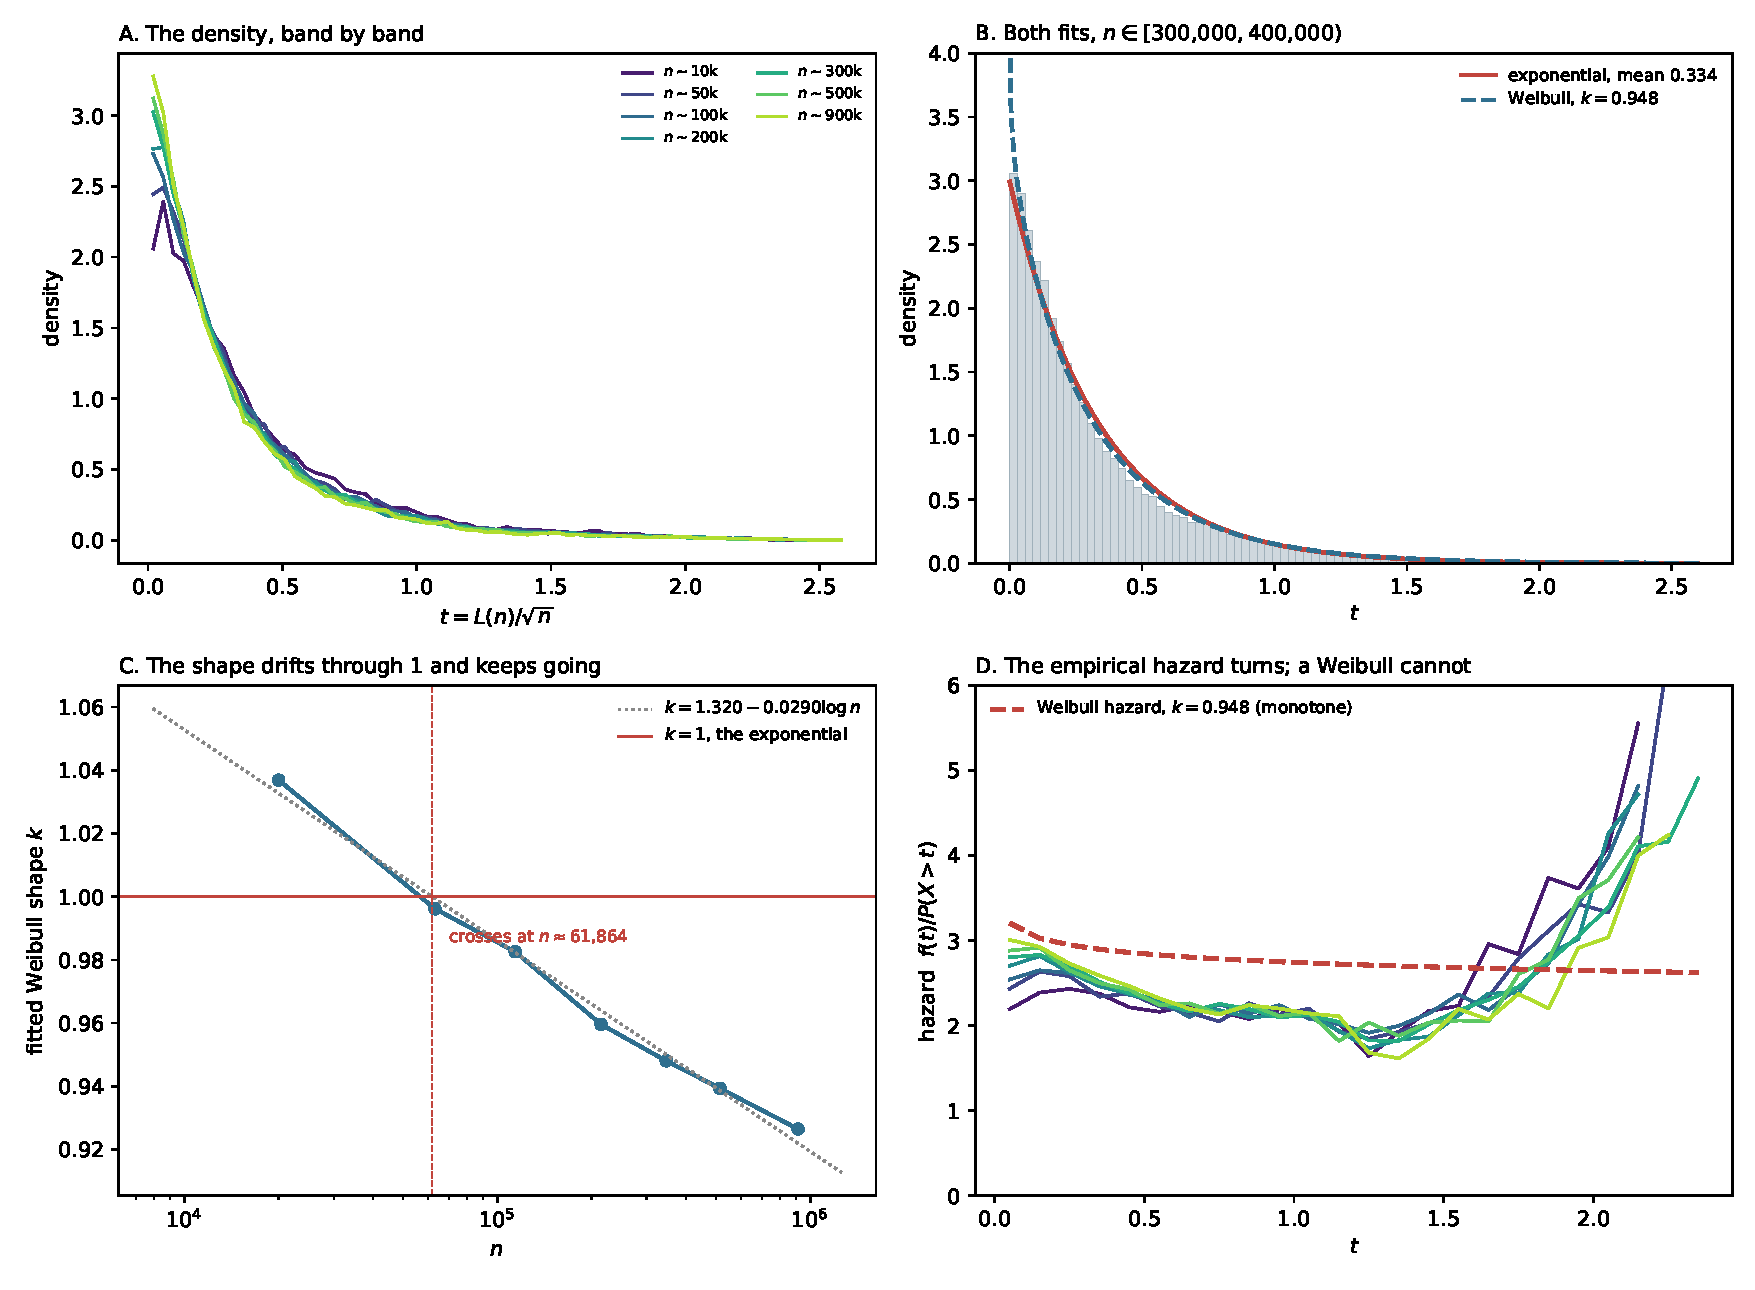
\includegraphics[width=\textwidth]{weibull-figure.pdf}
\end{center}

\section{What the two arms are}

The U has one mechanism per arm, and they are different.

The falling arm is a mixture. The period is essentially the regulator divided by the L\'evy constant $1.187$, and the spread across $n$ comes from the class number. A mixture of exponentials with varying rates always has a falling hazard --- the slow components survive longest, so survivors are drawn increasingly from them. Mixing cannot produce a rising hazard.

The rising arm must therefore be the edge. There is a ceiling, $L(n)=O(\sqrt n\log n)$; it is soft, and it drifts. As $t$ approaches it the survivors run out of room. No mixture supplies that.

A single-parameter family is being asked to represent two mechanisms pulling in opposite directions, and the balance between them moves with $n$ because the edge moves with $n$. That is why $k$ drifts, and why the drift has no limit in this data.

\section{Reproducing}

\begin{verbatim}
python3 weibull_sweep.py    # periods, fits, KS, hazards for all seven bands
python3 weibull_plots.py    # the four panels
tectonic weibull.tex
\end{verbatim}

The periods are recomputed from scratch in every band. As a check, the band $[3\times10^5,4\times10^5)$ reproduces $99{,}915$ non-squares, mean $0.3343$, shape $0.9480$ and KS distances $0.0346$ and $0.0210$, matching the September figures to four decimal places.

\end{document}
